16. \begin{figure}[ht!]
\center{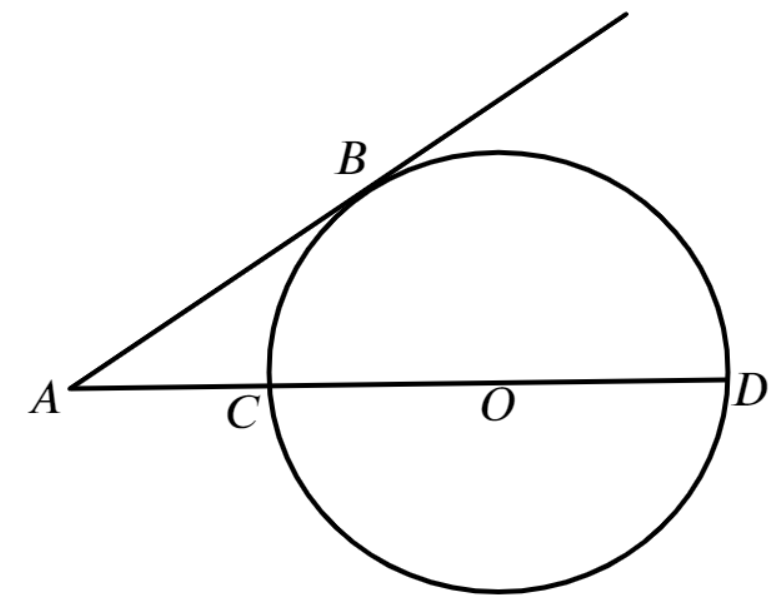
\includegraphics[scale=0.35]{g8-15.png}}
\end{figure}\\
По свойству касательной и секущей имеем $AB^2=AC\cdot AD.$ По условию $AD=3AB,$ значит $AB^2=AC\cdot3AB,\ AB=3AC.$ Пусть радиус окружности равен $x,$ тогда $AC=AD-2x,\ AC=3AB-2x,\ AC=9AC-2x,\ AC=\cfrac{1}{4}x.$ Поэтому $AB=3AC=\cfrac{3}{4}x,$ значит $x=\cfrac{4}{3}AB.$
ewpage
oindent
